\chapter[Árboles (*)]{Árboles (*)}\label{cap.arboles}

\begin{section}{Contando las hojas de un árbol con raíz}\label{seccion-arboles-con-raiz}
\label{6.1}

Recordemos que un {árbol} es un grafo conexo que no contiene ciclos. Los árboles aparecen en contextos diferentes y a menudo un vértice del árbol se distingue de los otros. Por ejemplo en el árbol genealógico que describe la descendencia de un rey, nosotros podemos enfatizar la posición especial del rey poniéndolo en lo
más alto del árbol. En general, nosotros llamaremos al vértice notable la \textit{raíz} del árbol, y a un árbol con una raíz \index{raíz} específica lo llamaremos \textit{árbol con raíz}. (Esta \index{árbol con raíz} terminología, aunque estándar, tiene el defecto que en la representación pictórica la raíz aparece en lo
más alto del árbol y el árbol 'crece' hacia abajo.)

Para el estudio de un árbol con raíz es natural ubicar los vértices en niveles, de la misma manera que lo hicimos para los grafos bipartitos en la sección \ref{seccion-algoritmo-greedy-para-coloreo}. Diremos que el vértice raíz es el \textit{nivel $0$} y que sus vecinos forman el \textit{nivel $1$}.  Para cada $k\ge 2$, el \textit{nivel $k$} está formado por aquellos vértices que son adyacentes a vértices del nivel $k-1$, excepto aquellos que ya pertenecen al nivel $k-2$. El árbol con raíz representado en la Fig. \ref{f6.1} puede ser dibujado nuevamente como se lo muestra a la derecha de manera de visualizar los niveles. \index{niveles de un árbol}

\begin{figure}[ht]
    \renewcommand{\varx}{1} % variable para cambiar coordenada x
    \renewcommand{\vary}{1} % variable para cambiar coordenada y
    \renewcommand{\varc}{1}
    \begin{center}
    \begin{tabular}{llllll}
        & 
        \begin{tikzpicture}[scale=1]
        %\SetVertexSimple[Shape=circle,MinSize=5 pt,FillColor=white]
        \Vertex[x=-2.00, y=0.00, L=$a$]{0}
        \Vertex[x=-1.00, y=0.00, L=$b$]{1}
        \Vertex[x=1.0, y=0.00, L=$c$]{2}
        \Vertex[x=0.00, y=-1.00, L=$r$]{9}
        \Vertex[x=0.00, y=-2.00, L=$g$]{6}
        \Vertex[x=-1.00, y=-3.00, L=$h$]{7}
        \Vertex[x=1.00, y=-3.00, L=$i$]{8}
        \Vertex[x=-2.00, y=-3.00, L=$d$]{3}
        \Vertex[x=-2.00, y=-2.00, L=$e$]{4}
        \Vertex[x=-1.00, y=-2.00, L=$f$]{5}
        \Edges(0,1,9,2,9,6,7,5,7,4,7,3)
        \Edges(6,8)
        \end{tikzpicture}
        &
        \qquad\quad
        & 
        \begin{tikzpicture}[scale=1.2]
        %\SetVertexSimple[Shape=circle,MinSize=5 pt,FillColor=white]
        \Vertex[x=0.00, y=0, L=$r$]{9}
        \Vertex[x=-1.00, y=-1.00, L=$b$]{1}
        \Vertex[x=0.0, y=-1.00, L=$c$]{2}
        \Vertex[x=1.00, y=-1.00, L=$g$]{6}
        \Vertex[x=-1.00, y=-2.00, L=$a$]{0}
        \Vertex[x=0.00, y=-2.00, L=$h$]{7}
        \Vertex[x=1.00, y=-2.00, L=$i$]{8}        
        \Vertex[x=-1.00 , y=-3.00, L=$f$]{5}
        \Vertex[x=0.00, y=-3.00, L=$e$]{4}
        \Vertex[x=1.00 , y=-3.00, L=$d$]{3}
        \Edges(0,1,9,2,9,6,7,5,7,4,7,3)
        \Edges(6,8)
        \end{tikzpicture}
        &
        \,
        &
        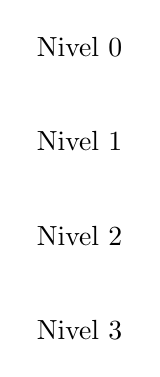
\begin{tikzpicture}[scale=1.2]
        \draw (0,0) node {Nivel 0};
        \draw (0,-1) node {Nivel 1};
        \draw (0,-2) node {Nivel 2};
        \draw (0,-3) node {Nivel 3};
        \end{tikzpicture}
    \end{tabular}
\end{center}
    \caption{Un árbol con raíz y sus niveles} \label{f6.1}
\end{figure}

Un vértice en un árbol con raíz se llama una \textit{hoja} si \index{hoja} pertenece al nivel $i$ ($i\ge 0$) y no es adyacente a ningún vértice del nivel $i+1$. Un vértice que no es una hoja es llamado \textit{interno}.  \index{vértice interno} La \textit{altura} de un árbol con raíz  \index{altura de un árbol con raíz} es el máximo valor de $k$ para el cual el nivel $k$ es no vacío. Luego el árbol de la Fig. \ref{f6.1} tiene seis hojas, cuatro vértices internos y su altura es tres.

Las dos propiedades que usamos en la sección \ref{seccion-arboles} para definir un árbol, ser un grafo conexo y sin ciclos, tienen consecuencias obvias cuando pensamos los vértices por niveles. Puesto que todo árbol es conexo entonces cada vértice pertenece a algún nivel. Más importante aún, puesto que un árbol no tiene ciclos  cada
vértice $v$ del nivel $i$ es adyacente a uno y solo uno $u$ del nivel $i-1$. A veces enfatizaremos esto diciendo que $u$ es el \textit{{padre}} de $v$ o que $v$ es un \textit{{hijo}} de $u$. Cada \index{padre de un vértice}  \index{hijo de un vértice} vértice, excepto el raíz, tiene un único padre, pero un vértice puede tener una cantidad arbitraria de hijos (incluso ninguno). Claramente, un vértice es una hoja si y solo si no tiene hijos.

En muchas aplicaciones ocurre que cada padre (vértice interno) tiene la misma cantidad de hijos. Cuando cada padre tiene $m$ hijos diremos que el árbol es \textit{$m$-ario}, en particular cuando $m=2$ diremos que el árbol es \textit{binario}  \index{árbol binario}  \index{árbol ternario} y cuando $m=3$ diremos que es \textit{ternario}.

\begin{teorema}\label{t6.1} La altura de un árbol con raíz $m$-ario con $l$ hojas es por lo menos $\log_ml$.
\end{teorema}
\begin{proof} Puesto que
$$
h \ge \log_ml \quad \Leftrightarrow \quad m^h \ge l
$$
es suficiente probar la afirmación equivalente: todo árbol con raíz $m$-ario de altura $h$ tiene a lo más $m^h$ hojas. La demostración es por inducción sobre $h$.

Claramente la afirmación es verdadera cuando $h=0$ puesto que en este caso el árbol es solo un vértice (la raíz) que es una hoja. Supongamos que la afirmación es verdadera cuando $0\le h \le h_0$ y sea $T$ un árbol con raíz $m$-ario de altura $h_0+1$. Si eliminamos la raíz y las aristas a las cuales pertenece obtenemos $m$ árboles $T_1,\ldots,T_m$ cuyas raíces son los vértices del nivel 1 de $T$. Cada $T_i$ es un árbol con raíz de altura $h_0$ o menos, luego por hipótesis inductiva tiene a lo más $m^{h_0}$ hojas. Pero las hojas de $T$ son precisamente las hojas de los árboles $T_1,\ldots,T_m$ y por consiguiente el número de hojas es a lo más $m \cdot m^{h_0}= m^{h_0+1}$.

Por el principio de inducción completa se sigue que la afirmación es verdadera para todo $h\ge 0$.
\end{proof}

Puesto que $\log_ml$ no es generalmente un número entero, el teorema anterior puede ser mejorado un poco. Por ejemplo si $m=3$ y $l=10$ la desigualdad
$$
h \ge \log_ml=2,0959\ldots
$$
implica que $h\ge 3$. En general podemos decir que
$$
h\ge\lceil \log_ml\rceil,
$$
donde $\lceil x \rceil$ denota el menor entero $z$ tal que $z\ge
x$.

Una aplicación frecuente del teorema \ref{t6.1} es en los  \index{árbol de decisión} \textit{árboles de decisión}. Cada vértice interno de un árbol de decisión representa una decisión y los posibles resultados de esa decisión son las aristas que unen ese vértice con los vértices del nivel siguiente. Los posibles  esultados finales del procedimiento son las hojas del árbol. Si el resultado de una decisión puede ser solo verdadero o falso entonces tenemos un árbol binario. A continuación daremos un ejemplo con un árbol ternario.

\begin{ejemplo} \label{monedafalsa}(El problema de la moneda falsa) Supongamos que tenemos una moneda genuina con la etiqueta $0$ y que tenemos otras $r$ monedas indistinguibles de $0$ por la apariencia excepto que tienen las etiquetas $1,2,\ldots,r$. Se sospecha que una moneda podría ser falsa, es decir o más liviana o más pesada. Probemos que son necesarias al menos $\lceil \log_3(2r+1)\rceil $ pesadas en una balanza para decidir que moneda (si hay alguna) es falsa y en ese caso ver si es más pesada o liviana. Mostremos un procedimiento que use exactamente este número de pesadas cuando $r=4$.
\end{ejemplo}
\begin{proof}[Solución] Hay $2r+1$ posibles resultados finales u hojas en el árbol de decisión: 
$$
B,1P,1L,\ldots,rP,rL;
$$
donde $B$ significa que todas las monedas son buenas, $iL$ significa que la moneda $i$ es más liviana y $iP$ que es más pesada. El árbol de decisión es ternario, puesto que hay tres posibles resultados de cada decisión (es decir de cada pesada entre un grupo de monedas y otro). Estos son:
\begin{alignat*}3
&<\quad & &:\quad& &\text{el grupo de la izquierda es más liviano}\\
&=\quad & &:\quad& &\text{los dos grupos pesan igual}\\
&>\quad & &:\quad& &\text{el grupo de la izquierda es más pesado.}
\end{alignat*}
Por consiguiente la altura del árbol de decisión es al menos $\lceil \log_3(2r+1)\rceil$.

Cuando $r=4$ entonces $\lceil \log_3(2r+1)\rceil=2$, y la solución con dos pesadas se gráfica en la Fig.\-\,\ref{f6.2}

\begin{figure}[ht]
    \begin{center}
    \begin{tikzpicture}[scale=1.2]
    {\renewcommand{\VertexShape}{rectangle}
        \Vertex[x=0.00, y=0, L ={\;$0,1 | 2,3$\;}]{0}
        \Vertex[x=-3, y=-1.5, L={$2|3$}]{1}
        \Vertex[x=0, y=-1.5, L={$0|4$}]{2}
        \Vertex[x=3, y=-1.5, L={\,$2|3$\,}]{3}
        \Vertex[x=-3.8, y=-3]{$3H$}
        \Vertex[x=-3, y=-3]{$1L$}
        \Vertex[x=-2.2, y=-3]{$2H$}
        \Vertex[x=-0.8, y=-3]{$4H$}
        \Vertex[x=0, y=-3]{$G$}
        \Vertex[x=0.8, y=-3]{$4L$}
        \Vertex[x=2.2, y=-3]{$2L$}
        \Vertex[x=3, y=-3]{$1H$}
        \Vertex[x=3.8, y=-3]{$3L$}
    }
    \SetVertexSimple[Shape=rectangle,FillColor=white,MinSize=8 pt]
    %\draw (0, 0) node {$\boxed{\text{Primera casa}}$};
    \Edges(0,1,0,2,0,3)
    \Edges(1,$3H$,1,$1L$,1,$2H$)
    \Edges(2,$4H$,2,$G$,2,$4L$)
    \Edges(3,$2L$,3,$1H$,3,$3L$)
    \end{tikzpicture}
    \end{center}
    \caption{Solución del problema de la moneda falsa cuando $r=4$}
    \label{f6.2}
\end{figure}

\end{proof}

\subsection*{$\S$ Ejercicios}
\begin{enumex}
\item En la siguiente tabla $n_5(h)$ es el número de árboles con raíz no isomorfos que tienen $5$ vértices y altura $h$. (Dos árboles con raíz son isomorfos si hay un isomorfismo de grafos, sin considerar la raíz, que lleva la raíz de uno en la del otro.) Verificar la tabla construyendo los ejemplos para cada caso.
$$
\begin{matrix}
h: &1 &2 &3 &4 \\
n_5(h): &1 &4 & 3 &1
\end{matrix}
$$
\item Si se consideran los árboles comunes (sin raíz), ¿cuál es el número de árboles no isomorfos con $5$ vértices? Hacer una lista y controlar que la lista del ejercicio anterior sea completa.

\item Construir dos árboles con raíz no isomorfos ambos con $12$ vértices, $6$ hojas y altura $4$.    
    
\item Suponer que se organiza un campeonato de fútbol-$5$ donde participan $20$ equipos. El cam\-peo\-na\-to es por eliminación simple y no hay empates. Cons\-truir un esquema para el torneo basado en un árbol con raíz y pruebar que son necesarias al menos $5$ rondas. 

\item ¿Cuál es la cota inferior en el número de pesadas necesarias en el problema de la moneda falsa (ver el ejemplo \ref{monedafalsa}) cuando son seis monedas? Desarrollar un esquema que logre este número de pesadas.

\item Considerar la siguiente variante del problema de la moneda falsa. Hay ocho monedas y sabemos que hay exactamente una que es más liviana. Todas las demás son genuinas pero no hay ninguna moneda con la etiqueta $0$. Encontrar una cota inferior teórica del número de pesadas necesarias para detectar la moneda falsa y probar que este número puede ser alcanzado.
\end{enumex}

\end{section}


\begin{section}{Árboles expandidos y el problema MST} \label{seccion-erboles-expandidos-mst}

\begin{definicion}
    Sea  $G=(V,E)$ es un grafo conexo y  $T$ es un subconjunto de $E$ tal que
    \begin{enumerate}[label=\textit{\alph*)}]
        \item  cada vértice de $G$ pertenece a una arista en $T$;
        \item  las aristas de $T$ forman un árbol.
    \end{enumerate}
    En este caso decimos que $T$ es un \textit{árbol expandido} para \index{árbol expandido} $G$.  
\end{definicion}
   Por ejemplo, un árbol expandido para el grafo de la Fig. \ref{f6.3} se indica con las líneas más gruesas.

Es fácil hacer ``crecer'' un árbol expandido: tome un vértice arbitrario $v$ del ``árbol parcial'' inicial y agregue aristas con un extremo en $v$ y el otro extremo que no pertenezca al árbol parcial inicial. El árbol expandido de la Fig. \ref{f6.3} puede construirse haciéndolo crecer desde el vértice $a$ y conectando los otros vértices en el orden $b$, $c$, $e$, $f$, $d$, $h$, $g$, usando las aristas $ab$, $ac$, $ae$, $cf$,  $fd$, $fh$, $hg$. En general, si hay $n$ vértices nosotros deberemos hacer $n-1$ pasos, después de los cuales tendremos $1+(n-1)=n$ vértices y $n-1$ aristas (el cual es el número correcto de acuerdo al teorema \ref{t5.5}).

\begin{figure}[ht]
    \begin{center}
        \begin{tikzpicture}[scale=1.2]
        \SetVertexSimple[Shape=circle,MinSize=5 pt,FillColor=white]
        \Vertex[x=0.00, y=0]{0}
        \Vertex[x=0.00, y=2.00]{1}
        \Vertex[x=1.90, y=0.62]{2}
        \Vertex[x=1.18, y=-1.62]{3}
        \Vertex[x=-1.18, y=-1.62]{4}
        \Vertex[x=-1.90, y=0.62]{5}
        \Edges(1,2,3,4,5,1)
        \Edges(5,0,c,2)
        \Edges(0,e,3)
        \Edges(0,c)
        \Vertex[x=0.59, y=0.19]{c}
        \Vertex[x=0.36, y=-0.49]{e}
        \tikzstyle{edge} = [draw,line width=2.5pt]
        \draw[edge] (5) -- (1) -- (2);
        \draw[edge] (1) -- (0) -- (e) -- (c) -- (e) -- (3) -- (4);
        \tikzstyle{edge} = [draw,line width=1pt]
        \draw[edge] (0) -- (c);
        \draw (0,2.3) node {$a$};
        \draw (-2.2, 0.62) node {$b$};
        \draw (2.2, 0.62) node {$e$};
        \draw (-0.2, -0.2) node {$c$};
        \draw (0.59, 0.5) node {$d$};
        \draw (0.66, -0.49) node {$f$};
        \draw (-1.48, -1.62) node {$g$};
        \draw (1.48, -1.62) node {$h$};
        \end{tikzpicture}
    \end{center}
    \caption{Un grafo y uno de sus árboles expandidos} \label{f6.3}
\end{figure}


Verifiquemos que el método siempre funciona: sea $S$ el conjunto de vértices del árbol parcial que se ha logrado en un paso intermedio, es decir que $S$ no es ni vacío ni todo $V$. Si no existe una arista que tenga un extremo en $S$ y el otro en el complemento $\overline{S}$, entonces no existe un camino entre $S$ y $\overline{S}$ y por lo tanto $G$ es disconexo, lo cual contradice las hipótesis. Por consiguiente siempre existe una arista disponible en cada etapa de la construcción.

Los árboles expandidos son útiles en muchos contextos. Por ejemplo, su\-pon\-ga\-mos que cierta cantidad de ciudades deben ser unidas de a pares por gasoductos de tal forma que quede una red de gasoductos conexa. Algunos pares de ciudades puede ser imposible unirlas por razones geográficas y cada posible conexión tiene asociada un costo de construcción. Formalmente, tenemos un grafo $G=(V,E)$ cuyos vértices son ciudades y sus aristas son las posibles conexiones. Además te\-ne\-mos una función $w$ de $E$ a $\mathbb N$ de tal forma que $w(e)$ representa el costo de cons\-truc\-ción de la arista $e$. Diremos que $G$ y $w$ es un \textit{grafo con pesos} y que $w$ es la \textit{función de pesos}. \index{grafo con pesos} \index{función de pesos}

En el problema del gasoducto lo que se pretende es construir una red conexa al mínimo costo. Un red de ese tipo corresponde a un árbol expandido $T$ para $G$ cuyo peso total 
$$
w(T) = \sum_{e \in T} w(e)
$$
es lo mas pequeño posible. Nos referiremos a este problema como el \textit{problema MST }(del inglés MST = minimum spanning tree = \index{MST}  \index{minimum spanning tree} árbol expandido mínimo) para el grafo con pesos $G$.  \index{árbol expandido mínimo}

Dado que los valores de $w$ son enteros positivos, claramente el problema MST debe tener solución, puesto que hay solo un número finito de árboles expandidos $T$ para $G$ y cada uno de ellos da un valor entero positivo $w(T)$. En otras palabras, existe un árbol expandido mínimo $T_0$ tal que 
$$
w(T_0) \le w(T)
$$
para todos los árboles expandidos $T$ de $G$. Sin embargo puede haber varios con la misma propiedad.

Un algoritmo simple para el problema MST se basa en aplicar la estrategia greedy al método explicado anteriormente. Específicamente: en cada paso se agrega la arista ``más barata'' que une un nuevo vértice al árbol parcial. (Si hay varias aristas con la misma propiedad se selecciona una de ellas.) Por ejemplo,
si en la Fig. \ref{f6.4} comenzamos con $u$, luego debemos agregar aristas en el orden $uv$, $ux$, $uy$, $yz$. Por otro lado, si comenzáramos por $y$, entonces agregamos las aristas en el orden $yz$, $yu$, $uv$, $ux$. 

\begin{figure}[ht]
    \begin{center}
    \begin{tikzpicture}[scale=1.2]
    \SetVertexSimple[Shape=circle,MinSize=5 pt,FillColor=white]
    \Vertex[x=0.00, y=2.00]{1}
    \Vertex[x=1.90, y=0.62]{2}
    \Vertex[x=1.18, y=-1.62]{3}
    \Vertex[x=-1.18, y=-1.62]{4}
    \Vertex[x=-1.90, y=0.62]{5}
    \Edges(1,2,3,4,5,1)
    \Edges(1,3,5,2,4,1)
    \tikzstyle{edge} = [draw,line width=2.5pt]
    \draw[edge] (1) -- (2) -- (1) -- (3) -- (1) -- (4) -- (5);
    \draw (0,2.3) node {$u$};
    \draw (-2.2, 0.62) node {$z$};
    \draw (2.2, 0.62) node {$v$};
    \draw (-1.48, -1.62) node {$y$};
    \draw (1.48, -1.62) node {$x$};
    \GraphInit[vstyle=Classic]
    \Edge[label=2](1)(2)
    \Edge[label=6](1)(5)
    \Edge[label=5](1)(4)
    \Edge[label=4](1)(3)
    \Edge[label=8](2)(5)
    \Edge[label=7](2)(4)
    \Edge[label=5](2)(3)
    \Edge[label=6](3)(5)
    \Edge[label=7](3)(4)
    \Edge[label=2](4)(5)
    \end{tikzpicture}
    \end{center}
    \caption{Un árbol expandido mínimo} \label{f6.4}
\end{figure}

El  algoritmo puede ser descripto informalmente en los siguientes pasos:
\begin{itemize}
\item Inicializar un árbol con un sólo vértice (elegido arbitrariamente).
\item Agrandar el árbol agregando una arista: entre las aristas que conectan al árbol con vértices que aún no están en el árbol, elegir una de peso mínimo.
\item Repetir el paso anterior hasta que todos los vértices estén en el árbol
\end{itemize}

Un primera impresión nos dice que sería bastante sorprendente que el algoritmo greedy funcione para el problema MST, especialmente cuando recordamos que el algoritmo greedy para el problema de coloración de vértices no siempre produce una coloración con el menor número posible de co\-lo\-res. Pero en el caso del problema MST se tiene más suerte.

\begin{teorema}\label{t6.2} Sea $G=(V,E)$ grafo conexo con función de pesos $w: E \to  \mathbb N$, y supongamos que $T$ es el árbol expandido para $G$ construido por el algoritmo greedy. Entonces 
$$
w(T) \le w(U) \nopagebreak
$$
para todo árbol expandido $U$ de $G$.
\end{teorema}
\begin{proof} Denotemos $e_1,e_2,\ldots,e_{n-1}$ las aristas de $T$ en el orden en que aplicamos el algoritmo greedy. Si $U=T$ el resultado es obviamente verdadero. Si $U\not=T$ entonces hay aristas de $T$ que no están en $U$ y supongamos que la primera es $e_k$. Denotemos $S$ el conjunto de vértices en el árbol parcial que se construye por el greedy justo antes de agregar $e_k$ y sea $e_k=xy$ donde $x$ está en $S$ e $y$ no está
en $S$. Puesto que $U$ es un árbol expandido existe un camino de $x$ a $y$ y si uno viaja a través de este camino encontrará una arista $e^*$ con un vértice en $S$ y el otro no. Ahora bien, cuando $e_k$ es seleccionada para $T$ en el algoritmo greedy, $e^*$ es también candidata a ser seleccionada, pero no lo es. Por consiguiente debemos tener que $w(e^*) \ge w(e)$. Si $e^*$ aparece en $T$, entonces por el razonamiento anterior es una arista que viene después (en el orden dado) de $e_k$.

El resultado de remover $e^*$ de $U$ y reemplazarla por $e_1$ es un árbol expandido $U_1$, para el cual
$$
w(U_1) = w(U) -w(e^*)+w(e_k) \le w(U).
$$
Más aún, la primera arista de $T$ que no está en $U_1$ aparece después de $e_k$ en el orden dado. En consecuencia podemos repetir el procedimiento obteniendo una sucesión de árboles expandidos $U_1,U_2,\ldots,$ con la propiedad que cada uno tiene una secuencia inicial de aristas en común con las aristas de $T$ más
larga que el anterior y además $w(U_i) \ge w(U_{i+1})$. El proceso termina cuando obtenemos un árbol expandido $U_r$ igual a $T$ y tenemos
$$
w(T)=w(U_r) \le w(U_{r-1}) \le \cdots \le w(U_1) \le w(U),
$$
como queríamos demostrar.
\end{proof}

En forma más detallada, el algoritmo puede ser implementado con el siguiente pseudocódigo:

\begin{minipage}{0.95\textwidth}
\noindent \textsc{Algoritmo de Prim}
\vskip .2cm
\begin{small}
\begin{verbatim}
# pre: G grafo con vértices 0,...,n y pesos w(i,j)
#      (w(i,j) = infinito si ij no es arista de G)
# post: devuelve F un MST de G
Q = [1,,...,n]  # lista de vértices aún no utilizados en el MST
S = [0] # lista de vértices ya utilizados en el MST
# L = [[k, 0, pesos[k][0]] : k en Q] 
# L se ira modificando de tal forma que si
# Q = [u0,...,uk] no utilizados en F 
# S = utilizados en F
# L  = [[ui,vi,w(ui,vi)]: 0 <= i <= k, vi in S tq w(ui,vi) mínimo]
F[i] = [],  0 <= i <= n # grafo con vértices 0,...,n y sin aristas.
while Q != []:
    L.sort(por coordenada 2) # ordena L por pesos 
    [u,v,p] = L[0]
    # u en Q, v en S, tal que p = w(u,v) es mínimo
    F.agregar_arista({u, v})
    L.remove([u, v, w(u,v)])
    Q.remove(u)
    S.append(u)
    for i in range(len(L)):
        u' = L[i][0]
        if w[u'][u] < L[i][2]:
            L[i][1] = u
            L[i][2] = w[u'][u]
    # el for actualiza la lista L
return F
\end{verbatim}
\end{small}
\end{minipage}

\vskip .5cm

Notemos que terminamos el proceso no cuando $S$ contiene todos los vértices, si no cuando, de manera equivalente, su complemento $Q$ queda vacío.   Existe una forma de ir viendo el progreso del algoritmo por medio de una tabla de tres columnas.
$$
\begin{matrix}
\text{I} &\text{II} & \text{III} \\
x & y & w(xy)\\
 .& .&. \\
. & .&. \\
. &. & .
\end{matrix}
$$

La Columna I lista los vértices que no están en $S$, que es el conjunto de vértices ya conectados al árbol parcial. Para cada $x$ en la Columna I la correspondiente entrada $y$ en la Columna II es un vértice en $S$ tal que la arista $xy$ es una de las aristas más baratas que unen el vértice $x$ con alguno de $S$. La  Columna III contiene el valor $w(xy)$.

En el $i$-ésimo paso de la construcción tenemos que $|S|=i$ y hay $n-i$ vértices en la Columna I. Tenemos entonces que seleccionar una de las entradas más pequeñas de la Columna III, digamos $w(x_0y_0)$, y esto conlleva $n-i-1$ comparaciones. Ahora debemos actualizar la tabla debido a que agregamos $x_0$ a $S$ por medio
de la arista $x_0y_0$. Primero debemos borrar la fila cuya primera posición tiene a $x_0$. Después en cada fila debemos verificar si la entrada correspondiente a la Columna II puede ser reemplazada por $x_0$ o no. Es decir para la fila $"x\quad y \quad w(xy)"$ debemos verificar si $xx_0$ es arista y si lo fuera y además $w(xx_0) < w(xy)$, entonces debemos reemplazar $y$ por $x_0$. Esto agrega otras $n-i-1$ comparaciones. El número total de comparaciones requeridas es
$$
\sum_{i=1}^{n-1} 2(n-i-1) = (n-1)(n-2).
$$
Esto nos dice que para encontrar un MST de un grafo deben hacerse alrededor de $n^2$ operaciones.

\subsection*{$\S$ Ejercicios}
\begin{enumex}
    \item Encontrar árboles expandidos para el cubo Fig. \ref{f5.12} y para el grafo de Petersen.

    \item Muestrar esquemáticamente todos los árboles expandidos del grafo completo $K_4$ (hay $16$).    

    \item Usar el algoritmo greedy para encontrar un MST del grafo representado en la Fig. \ref{f6.5}. ¿Es en este caso el MST único?
    \begin{figure}[ht]
    \begin{center}
    \begin{tikzpicture}[scale=1.8]
    %\SetVertexSimple[Shape=circle,MinSize=5 pt,FillColor=white]
    \Vertex[x=0.00, y=0.00, L = $a$]{1}
    \Vertex[x=1.5, y=1, L =$b$]{2}
    \Vertex[x=1.5, y=-0, L=$c$]{3}
    \Vertex[x=1.5, y=-1, L=$d$]{4}
    \Vertex[x=3, y=1, L =$e$]{5}
    \Vertex[x=3, y=-0, L=$f$]{6}
    \Vertex[x=3, y=-1, L=$g$]{7}
    \Vertex[x=4.5, y=1, L =$h$]{8}
    \Vertex[x=4.5, y=-0, L=$i$]{9}
    \Vertex[x=4.5, y=-1, L=$j$]{10}
    \Vertex[x=6, y=-0, L=$k$]{11}
    \Edge[label=2](1)(2)
    \Edge[label=8](1)(3)
    \Edge[label=1](1)(4)
    \Edge[label=6](2)(3)
    \Edge[label=7](3)(4)
    \Edge[label=1](2)(5)
    \Edge[label=1](3)(6)
    \Edge[label=9](4)(7)
    \Edge[label=2](5)(8)
    \Edge[label=6](6)(9)
    \Edge[label=1](7)(10)
    \Edge[label=9](8)(11)
    \Edge[label=2](9)(11)
    \Edge[label=4](10)(11)
    \Edge[label=5](3)(5)
    \Edge[label=1](3)(6)
    \Edge[label=2](3)(7)
    \Edge[label=3](5)(6)
    \Edge[label=4](6)(7)
    \Edge[label=9](5)(9)
    \Edge[label=3](7)(9)
    \Edge[label=7](8)(9)
    \Edge[label=1](9)(10)
    \end{tikzpicture}
    \end{center}
    \caption{Encontrar el MST} \label{f6.5}
\end{figure}

\item Sea $G$ un grafo con pesos cuyos vértices son $x,a,b,c,d,e,f$ y cuyas aristas y pesos vienen dados por la siguiente tabla:

\begin{align*}
xa &&xb &&xc &&xd &&xe &&xf &&ab &&bc &&cd &&de &&ef &&fa \\
6  &&3  &&2  &&4  &&3  &&7  &&6  &&2  &&3  &&1  &&8  &&6.
\end{align*}

Encontrar todos los árboles expandidos mínimos para $G$.

\item Suponer que $T$ es un árbol expandido mínimo en un grafo con pesos $K$ y sea $e^*$ una arista de $K$ que no es de $T$. Sea $e$ una arista de $T$ perteneciente al único camino en $T$ que une los vértices de $e^*$. Probar que $w(e) \le w(e^*)$. 

\item Escribir un ``programa'' para el algoritmo greedy basado en el
método ta\-bu\-lar mostrado más arriba.
\end{enumex}


\end{section}
